\chapter{Ecuaciones de \emph{Euler-Lagrange}}
\label{CapEEL}

	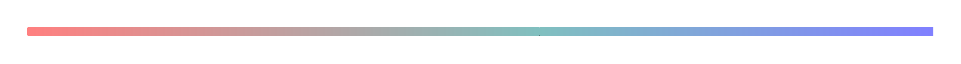
\begin{tikzpicture}
	\fill [left color=red!50, right color=teal!50] (0,0) rectangle (6.5,.1);
	\fill [left color=teal!50, right color=blue!50] (6.5,0) rectangle (11.5,.1);
	\end{tikzpicture}

\vspace{1cm}


\begin{adjustwidth}{50pt}{50pt}
\begin{ejemplo}
	Estudiaremos ahora el \emph{Principio de D'Alembert \textbf{dinámico}} y  deduciremos las ecuaciones \emph{Euler-Lagrange} como se hizo históricamente (no usando cálculo variacional).	
\end{ejemplo}
\end{adjustwidth}
	
\vspace{0.5cm}

\section{Principio de \emph{D'Alembert} dinámico}

\vspace{0.5cm}

\begin{myblock}{Principio de D'Alembert para el caso dinámico}
$\,$

\begin{Large}
\begin{equation}
\label{DAD}
 \displaystyle \sum_i \ \left( \dot{ \ \overrightarrow p_i}\ - \ \overrightarrow{F_i}^{(a)} \right ) \cdot \delta \overrightarrow{r_i}	 \ = \ 0
\end{equation}
\end{Large}
$\,$
\end{myblock}

Recuérdese que $\ \displaystyle \overrightarrow p =m\overrightarrow v\ $ es la cantidad de movimiento y  

$\displaystyle  \dot{\overrightarrow p}=\dv{t} (m\overrightarrow v) = \textcolor{gris}{(m=cte)} = m\dv{\overrightarrow v}{t}=m \overrightarrow a$ es la 2a ley de Newton.

Otra forma de escribir la ecuación \ref{DAD}, considerando la cantidad de movimiento es:

\begin{myalertblock}{Principio de D'Alembert para el caso dinámico}	
\begin{large}
\begin{equation}
\label{DAD2}
\boldsymbol{ \displaystyle \sum_i \ \left( m \overrightarrow a_i \ - \ \overrightarrow{F_i}^{(a)} \right ) \cdot \delta \overrightarrow{r_i}	 \ = \ 0 }
\end{equation}
\end{large}
\end{myalertblock}

En un sistema de partículas, el subíndice $\boldsymbol i$ hace referencia a cada una de las partículas que componen el sistema, en el caso de un sólido rígido, $\boldsymbol i$ hace referencia a ls puntos donde se aplican las fuerzas.

Resolveremos un mismo ejemplo-problema de tres formas distintas: 1 - por Newton, 2 - por D'Alembert y 3 - con las ecuaciones de Euler-Lagrange.

\vspace{1cm}
\begin{example}
.	Partícula que se mueve libremente a lo largo de una barra.

\begin{figure}[H]
	\centering
	\includegraphics[width=.6\textwidth]{imagenes/img02-01.png}
\end{figure}
\end{example}

\vspace{1cm}
\subsection{Resolución por \emph{Newton}}
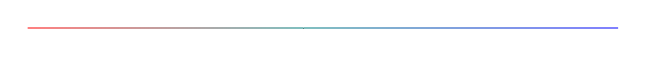
\begin{tikzpicture}
	\fill [left color=red!50, right color=teal!50] (0,0) rectangle (3.5,.01);
	\fill [left color=teal!50, right color=blue!50] (3.5,0) rectangle (7.5,.01);
	\end{tikzpicture}
	
\vspace{0.5cm}
Suponemos que no hay fricción. Las únicas fuerzas que actúan son el peso, $\overrightarrow P$, y una fuerza de reacción de la barra, que se opone al movimiento y es perpendicular a la superficie de contacto, $\overrightarrow T$. Usamos como sistema de referencia el centrado en la partícula que se mueve y cuyo eje x es solidario con la barra sobre la que se desplaza la partícula:

$\overrightarrow T=(0,T);\quad \overrightarrow P=(mg\sin \theta, -mg \cos \theta)$

Aplicando la 2a de Newton:

$\displaystyle \boldsymbol{ \sum_i  \overrightarrow F_i =m\overrightarrow a } \ \to \ (0,T)+(mg\sin \theta, -mg \cos \theta)=m\overrightarrow a$

$(mg\sin \theta, T-mg \cos \theta)=m(a_x,a_y) \ \to \ \begin{cases}
 \ a_x=g\sin \theta	 \\ \ a_y=(T-mg \cos \theta) / m
 \end{cases}$

Como a partícula está obligada a moverse a lo largo del eje x, no hay movimiento en el eje y: $\ a_y = 0 \ \to \ $

\begin{multicols}{2}
\begin{equation}
T \ = \ mg\cos \theta	
\end{equation}

\begin{equation}
a_x \ = \ g \sin \theta	
\end{equation}
\end{multicols}

Calculemos, ahora, el tiempo que tarda nuestra partícula en recorrer toda la barra, desde el punto A hasta el B.

$a_x=g\sin \theta = cte \ \to \ MRUA \ \to \ x=\cancelto{0}{x_0}+ \cancelto{0}{v_0}t+\dfrac 1 2 a_x t^2=\dfrac 1 2 g \sin \theta t^2$

De la figura, puesto que $\theta$ es el ángulo de un triángulo rectángulo de cateto opuesto $2$ y cateto contiguo $1$ (hipotenusa $\sqrt{5}$), se tiene que $\sin \theta = 2/\sqrt{5}$, tomando $g\approx 10$ ms$^{-2}$, obtenemos:

$x=\dfrac 1 2 \ 10 \ \dfrac 2 {\sqrt{5}} t^2 = \dfrac {12}{\sqrt
5} t^2$

Al recorrer la partícula toda la longitud de la barra, $\sqrt
5$, obtendremos finalmente que el tiempo empleado es: \textcolor{gris}{$\left( \sqrt{5}=\dfrac {12}{\sqrt
5} t^2 \ \to \ 5=10 t^2 \right)$}

\begin{equation}
\label{R2MN}
\subrayado{ \ \boxed{ \ 
	t \ = \ \dfrac 1 {\sqrt{2}} \ \mathrm{s}
\ } \ }
\end{equation}

\vspace{1cm}
\subsection{Resolución por \emph{D'Alembert}}
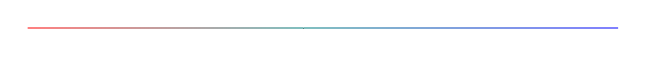
\begin{tikzpicture}
	\fill [left color=red!50, right color=teal!50] (0,0) rectangle (3.5,.01);
	\fill [left color=teal!50, right color=blue!50] (3.5,0) rectangle (7.5,.01);
	\end{tikzpicture}
%\vspace{0.5cm}

La única fuerza aplicada es el $\overrightarrow P$, la $	\overrightarrow T$ es una fuerza de ligadura (restrictiva), por lo que el principio de D'Alembert \emph{dinámico} dice que:

\begin{equation}
\label{PDDT2E}
\boldsymbol{
	( \ m\overrightarrow a \ - \ \overrightarrow P \ ) \ \cdot \ \overrightarrow {\var r	} \ =  \ 0
}
\end{equation}

%\vspace{5mm}
\begin{multicols}{2}
\begin{figure}[H]
	\centering
	\includegraphics[width=.4\textwidth]{imagenes/img02-02.png}
\end{figure}


Para calcular el desplazamiento virtual $\overrightarrow{\var r}$, vamos a \emph{parametrizar} la recta por la que está obligada a moverse la partícula: $\ y=ab+b$, que pasa por los puntos $A(0,2)$ y $B(1,0)$.

$A(0,2):\ \  2=a\cdot 0 + b \to b=2$

$B(1,0):\ \ 0=a\cdot 1 + 2 \to a=-2$

La recta buscada es: $\ y=-2x+2$ 
\end{multicols}



\begin{equation}
\label{paramT2}
\text{\emph{Parametrización:}}\quad 
\begin{cases}
\ x\ = \ q \\ \ y \ = \ -2q+2
\end{cases} ; \qquad q \in [0,1] \subset \mathbb R
\end{equation}

A medida que varía $q \in [0,1]$ variará la $\overrightarrow r$ y la partícula se moverá siempre por la barra.

$\begin{cases} 
	 \displaystyle \ \var x = \pdv{x}{q} \var q = 1\cdot \var q \\ \displaystyle \ \var y = \pdv{y}{q} \var q = -2  \cdot \var q
\end{cases} \to \quad \overrightarrow{\var r} = (1,-2) \ \var q $

Llevando este resultado y sabiendo que $\ \overrightarrow P=(0,-P)\ $ a la ecuación del principio de D'Alembert dinámico\ref{PDDT2E}, tenemos:

$(ma_x,ma_y-(-mg)) \cdot (1,-2) \ \var q =0 \to \cancelto{\neq 0}{m} \ (a_x-2(a_y+g)) \ \cancelto{\neq 0} {\var q} = 0$, por lo que

\begin{equation}
\label{R2PDD}
\boxed{ \ a_x \ = \ 2 (a_y+g) \ }	
\end{equation}

Relación que, de momento, no se asemeja demasiado al resultado obtenido aplicando la mecánica newtoniana, ec. \ref{R2MN}.

Vamos a derivar (dos veces) las ecuaciones de la parametrización, ec \ref{paramT2}:

$\begin{cases}
\ x =  q \\ \ y  = -2q+2
\end{cases} \to \qquad \begin{cases}
 \  \dot x = \dot q \\ \ \dot y = -2 \dot q
 \end{cases} \to \qquad \begin{cases}
 \ \ddot x= \ddot q =a_x	 \\ \ \ddot y=-2\ddot q = a_y
 \end{cases}$

Sustituyendo en ec. \ref{R2PDD}, tenemos: $\ \ddot q=2(-2\ddot q +g) \ \to \ 5\ddot q= 2g$, por lo que, con $g\approx 10 \ \mathrm{ms}^{-2}$,

\begin{equation}
\ddot q = 4	
\end{equation}

Integramos, ahora (dos veces) para encontrar $q(t)$

$\ddot q(t) = \displaystyle \int \ddot q \ \dd t = \int 4 \ \dd t = 4t +K$

$q(t)= \displaystyle \int \dot q \ \dd t = \int (4t+K) \ \dd t = 2t^2 +Kt+C$

Impongamos las condiciones iniciales:

$t=0: \ A(x=0,y=2)  \ \to \ q(0)=x(0)=0=2\cdot 0^2 + K\cdot o + C \to C=0$

$t=0: \ $ \begin{tiny} {(partícula se mueve libremente)} \end{tiny} $ \ \dot q(0)=v_x(0)=0 \ \to \ 0=4\cdot 0 + K \to K=0$

Luego, $\ q(t)=2t^2$ y, con ello,

\begin{equation}
\label{R3PDD}	
\begin{cases}
	\ x \ = \ \textcolor{gris}{q} \ = \ 2t^2 \\
	\ y \ = \ \textcolor{gris}{-2q+2} \ = \  -4t^2+2
\end{cases}
\end{equation}

Ecuaciones cuya solución es equivalente a la que hemos obtenido al aplicar la mecánica newtoniana.

Como comprobación, calcularemos el tiempo que tarda la partícula en recorrer toda la barra.

Al llegar al suelo, $\ y=0=-4t^2+2$, despejando:

\begin{equation}
\label{RFPDD}
\subrayado {\ \boxed{ \ \ t \ = \ \dfrac{1}{\sqrt{2}}	\ \mathrm{s} \ } \ }
\end{equation}

Resultado que, evidentemente, coincide con el obtenido con Newton, ec. \ref{R2MN}.

Parece que esto no sea más que complicarse absurdamente la existencia, pero en el caso de que hayan \emph{ligaduras}, el método de Newton es ardua, en cambio, \emph{parametrizando} el vector de posición respecto de unas variables que llamaremos \emph{``variables generalizadas''} hará que todo sea mucho más sencillo.

Vamos ahora a introducir las \emph{ecuaciones de Euler-Lagrange} que nos facilitarán aún más el cálculo y volveremos a resolver por tercera vez el problema-ejemplo de la partícula en la barra.


\vspace{1cm}
\section{Ecuaciones de \emph{Euler-Lagrange}}
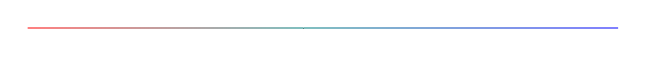
\begin{tikzpicture}
	\fill [left color=red!50, right color=teal!50] (0,0) rectangle (3.5,.01);
	\fill [left color=teal!50, right color=blue!50] (3.5,0) rectangle (7.5,.01);
	\end{tikzpicture}
\vspace{0.5cm}

Por sencillez, consideraremos el caso de solo una partícula cuya trayectoria se puede parametrizar con un solo parámetro (grado de libertad), q, que recibe n el nombre de \textbf{\emph{coordenadas generalizadas}}.

Vamos a pasar del principio de D'Alembert dinámico a las ecuaciones de Euler-Lagrange, partimos de:

$$\displaystyle \sum_i \left ( \ \dot{\ \overrightarrow p_i} - \overrightarrow F^{(a)}_i \ \right) \ \cdot \ \overrightarrow{\var r_i} \ = \ 0$$

De otro modo: $\qquad   (\dot{\ \overrightarrow p} - \overrightarrow F)\cdot \overrightarrow {\var r} = 0 \ \to \dot{\ \overrightarrow p}\cdot \overrightarrow{\var r} = \overrightarrow F \cdot \overrightarrow{\var r}$

El vector de posición dependerá del parámetro $q$ y, tal vez, del tiempo $t$: $\quad \overrightarrow r= \overrightarrow r (q,t)$.

\begin{small}
\textcolor{gris}{Obviamente, la parametrización ha de satisfacer las condiciones de ligadura:}

\textcolor{gris}{Circunferencia radio $R$: $\ \begin{cases} \ x=R \cos q \\ \ y=R \sin q \end{cases}$; $\quad$ Nuestra barra: $\ \ \begin{cases} \ x=q \\ \ y=-2q+2 \end{cases}$; $\quad$ etc.}
\end{small}


Como $\ \dot{\ \overrightarrow p}=m\dot{\ \overrightarrow v} \ \text{ y }  \ \displaystyle \overrightarrow{ \var r} = \pdv{\overrightarrow r}{q} \var q \ , \ \  \qquad m \dot{\ \overrightarrow v} \cdot \pdv{\overrightarrow r}{q} \var q = \overrightarrow F \cdot \pdv{\overrightarrow r}{q} \var q $

Por \textbf{definición}, llamamos \textbf{\emph{fuerza generalizada}}, $\boldsymbol {Q}$, a la expresión siguiente cuyo sentido encontraremos más adelante:

\begin{equation}
\label{T2FG}	
\boxed{ \ \overrightarrow F \ \cdot \ \pdv{\overrightarrow r}{q}\ =  \ Q \ }
\end{equation}

Con lo que, de momento, el principio de D'Alembert dinámico nos queda como:

\begin{equation}
\label{T2PDD2}
m \dot{ \ \overrightarrow v} \ \cdot \ 	\pdv{\overrightarrow r}{q} \ \ \overrightarrow{\var q} \ = \ Q\ \var q
\end{equation}

Analicemos la primera parte de esta ecuación, $\displaystyle \ m \dot{ \ \overrightarrow v}  \cdot 	\pdv{\overrightarrow r}{q}$, para $m=cte$,

$$\displaystyle m \dot{ \ \overrightarrow v} \cdot \pdv{\overrightarrow r}{q} = \dv{t} \, (m\overrightarrow v)\cdot \pdv{\overrightarrow r}{q}$$

Desarrollemos la expresión: $\displaystyle \ \ \dv{t} \left[ m \overrightarrow v \cdot \pdv{\overrightarrow r}{q} \right] = 
 \dv{t} \, (m\overrightarrow v)\cdot \pdv{\overrightarrow r}{q} +
 m \overrightarrow v \cdot \dv{t} \left( \pdv{\overrightarrow r}{q} \right)   $
 
 
 \begin{equation}
 \label{T2PDD3}
 \text{Despejando: } \qquad \qquad 
 \dv{t} (m\overrightarrow v) \cdot \pdv{\overrightarrow r}{q} \ = \ 	
 \dv{t} \left[ m \overrightarrow v \cdot \pdv{\overrightarrow r}{q} \right] -
 m \overrightarrow v \cdot \dv{t} \left( \pdv{\overrightarrow r}{q} \right)
 \end{equation}

 
\rule{150pt}{0.1pt}

\underline{Inciso 1}:  $\quad$ como $\displaystyle \ \ \overrightarrow v= \dv{t} \overrightarrow r(q,t)= \pdv{\overrightarrow r}{q} \ \dv{q}{t} + \pdv{\overrightarrow r}{t}$

\textcolor{gris}{Ejemplo: $\ x=q^2+\sin t \to v=2q\dv{q}{t}+\cos t=2q\dot q+\cos t$}

\textcolor{gris}{Es como la regla de la cadena: $\ \dv{x}{t} = \dv{t} (q^2) + \dv{t} (\sin t) = 2q\dot q + \cos t$}

\begin{flushright}
\rule{200pt}{0.1pt}	
\end{flushright}

Teniendo en cuenta lo visto en el inciso 1,

\begin{equation}
\label{T2PDD4}
\boldsymbol{ \overrightarrow v \ = } \ \textcolor{gris}{ \dv{\overrightarrow r}{t} } \ \boldsymbol{ = \ \pdv{\overrightarrow r}{q}\ \dot q \  + \   \pdv{\overrightarrow r}{t} }
\end{equation}

Derivando respecto de $\dot q$: $\quad \displaystyle \pdv{\overrightarrow v}{\dot q} \ = \ \pdv{\dot q} \left( \pdv{\overrightarrow r}{q} \ \dot q \right) + \pdv{\dot q} \left(\pdv{\overrightarrow r}{t} \right) $

Aplicamos el \emph{teorema de Schwarz} para funciones continuas con derivadas continuas: `se puede cambiar el orden de derivación':

$\displaystyle \pdv{\overrightarrow v}{\dot q} \ = \ \pdv{\dot q} \left( \pdv{\overrightarrow r}{q} \ \dot q \right) + \pdv{ t} \cancelto{0}{\left(\pdv{\overrightarrow r}{\dot q} \right)} \, , \ \ $ ya que $\overrightarrow r=\overrightarrow r(q,t) \to  \neq \overrightarrow r(\dot q)$

Así pues, $\quad \displaystyle \boldsymbol{ \pdv{\overrightarrow v}{\dot q} } \ = \ \pdv{\dot q} \left( \pdv{\overrightarrow r}{q} \ \dot q \right) =
\cancelto{0}{\pdv{\dot q} \left( \pdv{\overrightarrow r}{q} \right)} \dot q + \pdv{\overrightarrow r}{q} \ \cancelto{1}{\pdv{\dot q}{\dot q} } = \boldsymbol{ \pdv{\overrightarrow r}{q} }$

Donde hemos tenido en cuenta la derivada del producto y que como

$\displaystyle \overrightarrow r = \overrightarrow r(q,t) \to \pdv{\overrightarrow r}{t}=\pdv{\overrightarrow r}{t} \ (q,t) \neq  \pdv{\overrightarrow r}{t} \ (\dot q)$%\ (q,t) \neq \pdv{\overrightarrow r}{t}  \ (\dot q)$

\begin{multicols}{2}
Destacamos este último resultado:	

\begin{equation}
\label{T2UR1}
\pdv{\overrightarrow v}{\dot q} \ = \ \pdv{\overrightarrow r}{q} 
\end{equation}
\end{multicols}

\rule{150pt}{0.1pt}

\underline{Inciso 2}:  $\quad \text{como: } \ \ \displaystyle \dv{t} \ A \ = \ \pdv{A}{B} \cdot \dv{B}{t} \ + \ \pdv{A}{t} $ , 

invirtiendo el orden $\displaystyle \dv{t} \ A \ = \ \dv{B}{t} \cdot  \pdv{A}{B} \ + \ \pdv{A}{t} \ $ y tomando $\ A=\displaystyle \pdv{\overrightarrow r}{q};\ \ B=q$,
$\displaystyle 	\dv{t} \ \left( \pdv{\overrightarrow r}{q}\right) 
= \dv{q}{t} \cdot \pdv{q} \left( \pdv{\overrightarrow r}{q} \right)  +
\pdv{t} \left( \pdv{\overrightarrow r}{q}  \right)=
\dot q \cdot \pdv{q} \left( \pdv{\overrightarrow r}{q} \right)  +
\pdv{q} \left( \pdv{\overrightarrow r}{t}  \right)$

donde hemos aplicado al último término el teorema de Schwarz.

Teniendo en cuenta la derivada de la suma y que $\ \dot q \neq \dot q(q)$,

$\displaystyle 	\dv{t} \ \left( \pdv{\overrightarrow r}{q}\right) 
= \pdv{q} \left( \dot q \ \pdv{\overrightarrow r}{q} \right) + \pdv{q} \left( \pdv{\overrightarrow r}{t} \right) =
\pdv{q} \left[ 
\dot q \ \pdv{\overrightarrow r}{q} + \pdv{\overrightarrow r}{t} \right]= \pdv{\overrightarrow v}{q} $

En la última igualdad hemos tenido en cuenta la ecuación \ref{T2PDD4}

\begin{flushright}
\rule{200pt}{0.1pt}	
\end{flushright}

\begin{multicols}{2}
Destacamos, también, este último resultado:	

\begin{equation}
\label{T2UR2}
\dv{t} \ \left( \pdv{\overrightarrow r}{q}\right) \ = \ \pdv{\overrightarrow v}{q}
\end{equation}
\end{multicols}

Volviendo, con estos resultados ( ec. \ref{T2UR1} y ec. \ref{T2UR2} ), a la ecuación \ref{T2PDD3}, en que analizábamos un trozo del primer miembro de la aplicación del principio de D'Alembert dinámico para una coordenada generalizada y una fuerza generalizada, tenemos:

\begin{equation}
\label{T2PDD6}
\displaystyle \dv{t} \ (m\overrightarrow v) \cdot \pdv{\overrightarrow r}{q}=
\dv{t} \left[ m\overrightarrow v \cdot \pdv{\overrightarrow v}{\dot q} \right]-
m\overrightarrow v \cdot \pdv{\overrightarrow v}{q}\ \ \ 
\quad \text{ Ya lo tenemos casi.}
\end{equation}

\rule{150pt}{0.1pt}

\underline{Inciso 3}.  Truco: derivada del producto.

$\displaystyle \pdv{a} \ (\vec v \cdot \vec v) = \pdv{\vec v}{a} \cdot \vec v + \vec v \cdot \pdv{\vec v}{a} = 2 \vec v \cdot \pdv{\vec v}{a}$

es decir, $\displaystyle \ \vec v \cdot \pdv{\vec v}{a} = \dfrac 1 2 \pdv{a} \ ( \vec v \cdot \vec v )= \dfrac 1 2 \pdv{a} ( |\vec v|\ |\vec v|\cos 0^o )  = \dfrac 1 2 \pdv{a} \ v^2$


multiplicando por $\displaystyle m\ \ \ m \vec v \cdot \pdv{\vec v}{a} = m \dfrac 1 2 \pdv{a} v^2 = \ \textcolor{gris}{(m=cte)} \ = \dfrac 1 2 \pdv{a} (\dfrac m 2 v^2)$

\begin{flushright}
\rule{200pt}{0.1pt}	
\end{flushright}

Aplicando el resultado del inciso 3 al caso $ \ \displaystyle a=\dot q \  \to \  m\vec v \cdot \pdv{\vec v}{\dot q}= \pdv{\dot q} \left( \dfrac 1 2 m v^2 \right) $

Aplicando el resultado del inciso 3 al caso $ \ \displaystyle a= q \  \to \  m\vec v \cdot \pdv{\vec v}{ q}= \pdv{ q} \left( \dfrac 1 2 m v^2 \right) $

Incorporando estos resultados a la ec. \ref{T2PDD6}, tenemos:

$\displaystyle \dv{t} (m\vec v) \cdot \pdv{\vec r}{q} = \dv{t}
\left( \pdv{\dot q} \left( \dfrac 1 2 m v^2 \right) \right)-
\pdv{q} \left( \dfrac 1 2 m v^2 \right)$

Llamando $T$, \textbf{\emph{energía cinética}} a $\quad \boldsymbol{T \ = \ \dfrac 1 2 \ m v^2}\ ,$

$\displaystyle \dv{t} (m\vec v) \cdot \pdv{\vec r}{q} \ = \ \dv{t} \left[ \pdv{T}{\dot q} \right] - \pdv{T}{q}$

Volviendo al principio, ec \ref{T2PDD2}, principio de D'Alembert dinámico con una coordenada generalizada y una fuerza generalizada,

$\displaystyle \left[
\dv{t} \left( \pdv{T}{\dot q} \right) - \pdv{T}{q}
\right] \ \var q \ = \ Q \ \var q\ .\quad$ Como $\ \var q \neq 0\ ,$

\begin{equation}
\label{T2PDD7}
\boxed{ \ 
\dv{t} \left( \pdv{T}{\dot q} \right) \ - \ \pdv{T}{q} \ = \ Q \ = \ \overrightarrow F \cdot \pdv{\vec r}{q}	
\ }
\end{equation}

Ecuación válida para una partícula con un sólo grado de libertad, q (una sóla coordenada generalizada). Es válida para cualquier fuerza aplicada (aún de fricción), no solo para fuerzas conservativas aunque sean estas las más interesantes desde el punto de vista de la física teórica, por ello, veamos el caso de que la fuerza aplicada sea conservativa.

\vspace{1cm}
\subsection{Ecuaciones de \emph{Euler-Lagrange} para el caso conservativo}
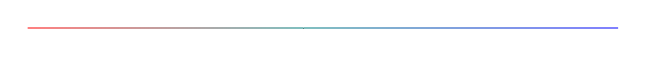
\begin{tikzpicture}
	\fill [left color=red!50, right color=teal!50] (0,0) rectangle (3.5,.01);
	\fill [left color=teal!50, right color=blue!50] (3.5,0) rectangle (7.5,.01);
	\end{tikzpicture}
\vspace{0.5cm}


Es sabido que en un caso conservativo\footnote{Aclaración al final del capítulo.}, $\overrightarrow \nabla \times \overrightarrow F = \overrightarrow 0 \ \to \ \overrightarrow F = - \overrightarrow \nabla V$, la fuerza proviene de un potencial escalar $V(\overrightarrow r, t)$, $\displaystyle \ \overrightarrow F = -\left( \pdv{V}{x},\pdv{V}{y},\pdv{V}{z} \right)$

$\displaystyle \overrightarrow F \cdot \pdv{\overrightarrow r}{q} = - 
\left( \pdv{V}{x} \pdv{x}{q},\pdv{V}{y} \pdv{y}{q},\pdv{V}{z} \pdv{z}{q} \right) = - \pdv{V}{q}\ , \ \ $ por la regla de la cadena. 

Por ello, $\ \displaystyle \dv{t} \left[ \pdv{T}{\dot q} \right] - 	\pdv{T}{q}=-\pdv{V}{q} \ \to \ \dv{t} \left[ \pdv{T}{\dot q} \right] - 	\left( \pdv{T}{q}-\pdv{V}{q} \right) =0$

Es decir, $\ \displaystyle \dv{t} \left[ \pdv{T}{\dot q} \right] -\pdv{q} (T-V)=0$, como $V=V(\overrightarrow r, t)=V(q,t) \neq V(\dot q)$, tendremos que $\displaystyle \pdv{V}{\dot q}=0$ y podremos escribir:
$\ \displaystyle \dv{t} \left[ \pdv{(T-V)}{\dot q} \right] -\pdv{(T-V)}{q}=0$

\vspace{1cm} %********
Se define el \textbf{lagrangiano} como $\ \boldsymbol {L=T-V}\, , \ $ con lo que las 	\textbf{ecuaciones de Euler-Lagrange} para \textbf{fuerzas conservativas} es:

\begin{equation}
\label{T2EEL1C}
\subrayado{ \ \boxed{ \ \boldsymbol{
\dv{t} \left[ \pdv{ L }{\dot q} \right] \ - \ \pdv{L}{q} \ = \ 0	
\ } \ } \ }
\end{equation}


\vspace{1cm}
\subsection{Extensión de las ecuaciones de \emph{Euler-Lagrange} para el caso de $\boldsymbol N$ partículas y $\boldsymbol n$ grados de libertad (ligaduras)}
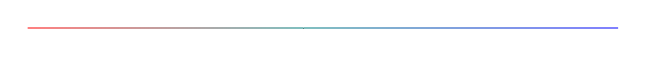
\begin{tikzpicture}
	\fill [left color=red!50, right color=teal!50] (0,0) rectangle (3.5,.01);
	\fill [left color=teal!50, right color=blue!50] (3.5,0) rectangle (7.5,.01);
	\end{tikzpicture}
\vspace{0.5cm}

$\displaystyle T=\sum_{i=1}^N \dfrac 1 2 m_i v_i^2 \ ; \qquad V=\sum_{i=1}^N V_i\, . \qquad  $Tendremos $\boldsymbol n$ ecuaciones del tipo:

\begin{myblock}{Ecuaciones Euler-Lagrange, caso conservativo}
\begin{large}
	\label{EELconservativas}
	\begin{equation}
	\dv{t} \left[ \pdv{ L }{\dot q_i} \right] \ - \ \pdv{L}{q_i} \ = \ 0	\, ; \quad i=1,2,\cdots n
	\end{equation}
\end{large}
\end{myblock}

En el caso general de fuerzas no conservativas,

\begin{myblock}{Ecuaciones Euler-Lagrange, caso general}
\begin{large}
	\begin{equation}
	\dv{t} \left[ \pdv{ L }{\dot q_j} \right] \ - \ \pdv{L}{q_j} \ = \ \sum_{j=1}^N\overrightarrow F_i \cdot \pdv{\overrightarrow r_i}{q_j} \, ; \quad j=1,2,\cdots n
	\end{equation}
\end{large}
\end{myblock}


%********************************************************
\vspace{1.5cm}

\begin{myexampleblock}{Observaciones}

\begin{itemize}
\item El movimiento del sistema lo determina una función escalar, el \emph{lagrangiano} en vez de cantidades vectoriales como en mecánica newtoniana.
\item Existe una ecuación para cada grado de libertad: la elección de las coordenadas generalizadas libres conduce directamente al número de ecuaciones del movimiento.
\item En las ecuaciones de Euler-Lagrange intervienen solo las fuerzas activas, no son tenidas en cuenta las que no realizan trabajos virtuales (T, N, ... ) que sí lo son en mecánica newtoniana.
\item Las ecuaciones de movimiento que se obtienen son ecuaciones diferenciales de segundo orden. Las constantes de integración las determinarán las condiciones iniciales.
\end{itemize}
\end{myexampleblock}


\vspace{1cm}

\begin{small}
\begin{myexampleblock}{Los campos vectoriales conservativos derivan de un potencial escalar}	

\begin{scriptsize}
\vspace{2mm} En una determinada región del espacio existe un \emph{campo de fuerza} cuando por el hecho de situar en cualquier parte de esta región un cuerpo, \emph{instantáneamente} aparece sometido a una fuerza.

\vspace{2mm} En `teoría clásica de campos' la interacción entre cuerpos del universo es \emph{instantánea}. La `teoría relativista de campos'  no permite la interacción instantánea, ninguna interacción se propaga a velocidad superior a la de la luz en el vacío, $c$.

\vspace{2mm} Llamamos \emph{magnitud activa de campo, $M$}, a la propiedad que tienen los cuerpos al interaccionar con los campos: $m$ en la interacción gravitatoria, $q$ en la eléctrica, .... Si $\vec E$ es la intensidad del campo en cuestión, $\vec F=M\ \vec E$.
\end{scriptsize}

\vspace{2mm} \textbf{Campos conservativos.}

\begin{multicols}{2}
Un campo es conservativo si el trabajo realizado por las fuerzas del campo para desplazar la magnitud activa $M$ del campo desde una posición $A$ hasta una posición $B$ es \ul{independiete del camino recorrido}, depende solamente de las posiciones inicial y final.
\begin{figure}[H]n
		\centering
		\includegraphics[width=.25\textwidth]{imagenes/img02-11.png}
		\caption*{\scriptsize{Campo conservativo: W depende solo de $A$ y $B$}\normalsize{.}}
		\end{figure}
\end{multicols}

\begin{multicols}{2}
\begin{figure}[H]
		\centering
		\includegraphics[width=.25\textwidth]{imagenes/img02-12.png}
		\caption*{\footnotesize{Campo central}\normalsize{.}}
		\end{figure}
Un caso particular de campo conservativo muy importante es el \emph{campo central:} cuando se deposita una magnitud activa en el campo aparecen sobre ella las fuerzas del campo que están dirigidas hacia el \emph{centro de fuerzas} y suelen ser \emph{inversamente proporcionales al cuadrado de la distancia} de la posición que ocupa la magnitud activa al el centro de fuerzas.
\end{multicols}

\vspace{2mm} \emph{\underline{Un campo de fuerzas central es necesariamente conservativo.}} Al ser central solo depende de la posición del centro de fuerzas y varía con la distancia (no necesariamente como $1/r^2$), veamos que es conservativo:

\vspace{2mm} Sea $M$, la magnitud activa del campo central $\vec E$, $\ \vec F=M \; \vec E= M \; \vec u_r \; \varphi(r)$, donde $\vec u_r=\dfrac {\vec r}{r}$ es un vector unitario que apunta al centro de fuerzas desde la posición que ocupe la magnitud activa y $\varphi(r)$ es la forma en que varía $\vec E$ con la distancia al centro de fuerzas.

\vspace{2mm}  Calculemos el trabajo necesario para desplazar la magnitud activa $M$ bajo la acción del campo central $\vec E$ desde un punto $A$ hasta otro $B$.
 
\vspace{2mm}  $\displaystyle W=\int_A^B \overrightarrow F \cdot \dd \vec r =\int_A^B M\; \varphi(r) \;\vec u_r \cdot \dd r= \int_A^B M\; \varphi(r) \; \dfrac {\vec r}{r} \cdot \dd r =(*) \int_A^B M\; \varphi(r) \; \dfrac {\cancel{r}\;\dd r}{\cancel{r}}=\int_A^B M\; \varphi(r)\; \dd r=(**)\eval{\Phi(r)}_{A}^B=\Phi(B)-\Phi(A)$
 
 \vspace{2mm}
 \textcolor{gris}{
 $(*)\quad \vec r\cdot \dd \vec r=r\;\dd r \cos 0^o=r\; \dd r $}
 
\textcolor{gris}{
 $(**)\quad \mathcal A\; \varphi(r)$ depende solo de $r$ y su primitiva será de la forma $\Phi(r)$ }

\vspace{2mm} Luego ``todo campo central es conservativo'' ya que el $W$ depende solo de las posiciones inicial $A$ y final $B$ y no del camino seguido. $\qquad \square$

\vspace{2mm} \textbf{Energia Potencial. Concepto de gradiente}

\vspace{2mm} Definición de energía potencial: \emph{El trabajo que realiza un campo de fuerza \underline{conservativo} al desplazar un cuerpo desde un punto $A$ hasta un punto $B$ es igual a la diferencia de energías potenciales existentes en los puntos $A$ y $B$.}

\begin{equation}
\label{Ener-poten}
W_{A\to B}=\int_A^B \vec F \cdot \dd \vec r = \mathcal E_p(A)- \mathcal E_p(B)\; \qquad \textcolor{gris}{(\vec F\; \text{conservativa})}	
\end{equation}

Esto que llamamos energía potencial $ \mathcal E_p$ es una función escalar característica del campo conservativo.

\vspace{2mm}
\rule{150pt}{0.4pt} 

\textbf{Otra definición de `campo conservativo':} 

\begin{multicols}{2}
$\,$

\emph{En un campo conservativo, el trabajo a lo largo de una trayectoria cerrada es cero.}
\begin{figure}[H]
		\centering
		\includegraphics[width=.3\textwidth]{imagenes/img02-13.png}
		\end{figure}
\end{multicols}

$W_{A\to A}=W_{A\to B}+W_{B \to A}=\mathcal E_p(A)-\mathcal E_p(B) \;+ \; \mathcal E_p(B)-\mathcal E_p(A)=0$

$$ \text{Campo conservativo:}\qquad \oint \vec F \cdot \dd \vec r =0$$

\textcolor{gris}{$\oint$ representa a la integral curvilínea cerrada.}

\rule{150pt}{0.4pt} 

\vspace{2mm}
\begin{equation}
\int_A^B \vec F \cdot \dd \vec r = \mathcal E_p(A)- \mathcal E_p(B)=-\int_A^B\dd \mathcal E_p	
\end{equation}

\begin{multicols}{2}
$\dd r = \dd l$, en la dirección de movimiento

$\vec F\cdot \dd \vec r=F\; \dd l\; \cos \theta =-\dd \mathcal E_p $

$F \cos \theta=- \dfrac{\dd \mathcal E_p}{\dd l} \; \to \;\; \vec u_r\;F \cos \theta=-\vec u_r\; \dfrac{\dd \mathcal E_p}{\dd l}$
\begin{figure}[H]
		\centering
		\includegraphics[width=.4\textwidth]{imagenes/img02-14.png}
		\end{figure}
\end{multicols}

\vspace{2mm}
$F\cos \theta$ es la componente de la fuerza en la dirección del movimiento, por ello, si conocemos $\mathcal E_p(x,y,z)$, podemos conocer la componente de $\overrightarrow F$ en cualquier dirección a partir de la cantidad $-\dd \mathcal E_p / \dd l$. Esto es lo que se llama \emph{derivada direccional} de $\mathcal E_p$. Cuando un vector es tal que su componente en una dirección determinada es igual a la derivada direccional de una función escalar en esa dirección, al vector se le llama \emph{gradiente} de la función escalar: $\vec F=-grad\;( \mathcal E_p)$

\vspace{2mm} Cuando estamos interesados en las componentes rectangulares de $\overrightarrow F$, la expresión $F \cos \theta$ es $F_x$, $F_y$ y $F_z$ y el desplazamiento $\dd l$ será $\dd x$, $\dd y$, y $\dd z$, de modo que:

\vspace{2mm} $\displaystyle F=\vec i\; F_x +\vec j\; F_y +\vec k\; F_z; \qquad F_x=- \pdv{\mathcal E_p}{x};\; F_y=- \pdv{\mathcal E_p}{y};\; F_z=- \pdv{\mathcal E_p}{z}$


\vspace{2mm}$\displaystyle \vec F=-\left[\;\vec i\;\;\pdv{\mathcal E_p}{x} + \vec j\;\;\pdv{\mathcal E_p}{y} + \vec k\;\;\pdv{\mathcal E_p}{z}\; \right]$

\vspace{2mm}
\begin{equation}
\displaystyle \vec F=- \left( \;\vec i\;\;\pdv{x} + \vec j\;\;\pdv{y} + \vec k\;\;\pdv{z}\; \right)\; \mathcal E_p
\end{equation}

\vspace{2mm}
Si llamamos `gradiente' al operador \emph{nabla}: $\displaystyle \grad= \vec i\;\;\pdv{x} + \vec j\;\;\pdv{y} + \vec k\;\;\pdv{z}$

\vspace{2mm}
\begin{equation}
\label{Ep-gradiente}
\vec F=-\overrightarrow{ \grad } \mathcal E_p	
\end{equation}

\vspace{2mm}
\emph{La energía potencial es característica de los campos conservativos.} 
En campos no conservativos no tiene sentido hablar de energía potencial.

\vspace{2mm}
$\displaystyle \pdv{F_x}{y}=-\pdv{\mathcal E_p}{y}{x} \quad = \quad -\pdv{\mathcal E_p}{x}{y}=\pdv{F_y}{x} \quad \to \quad \pdv{F_x}{y}-\pdv{F_y}{x}=0$ 

\vspace{2mm} Esto se cumple, por analogía, para las tres componentes:

\vspace{2mm} $\displaystyle \pdv{F_z}{y}-\pdv{F_y}{z}=0 \; \textcolor{gris}{\to\;  \vec i}\;;\quad \pdv{F_z}{x}-\pdv{F_x}{z}=0 \;\textcolor{gris}{\to\;  \vec j}\;;\quad \pdv{F_y}{x}-\pdv{F_x}{y}=0 \;\textcolor{gris}{\to\;  \vec k}$

\vspace{2mm} Y estas son las 3 condiciones que permiten definir matemáticamente a un campo conservativo: \emph{Un campo $\vec F$ es conservativo sus componentes satisfacen simultáneamente las tres ecuaciones anteriores.}

\vspace{2mm} Si lo escribimos vectorialmente:

\vspace{2mm} $\displaystyle \left( \pdv{F_z}{y}-\pdv{F_y}{z} \right) \;  \vec i+
\left( \pdv{F_z}{x}-\pdv{F_x}{z} \right) \;  \vec j+
\left( \pdv{F_y}{x}-\pdv{F_x}{y} \right) \;  \vec k\;$,

\vspace{2mm} que podemos escribir como:

\vspace{2mm} $\displaystyle \left| \begin{matrix} \vec i&\vec j&\vec k \\ \pdv{x}&\pdv{y}&\pdv{z} \\ F_x&F_y&F_z  \end{matrix} \right|=0 \to \overrightarrow{\grad } \times \vec F = 0$, si hacemos uso del operador nabla.

\vspace{2mm} Cuando el operador nabla actúa como producto vectorial sobre un vector se le llama \textbf{\emph{rotacional}}.


\vspace{2mm} $$\vec F \text{ es conservativo } \leftrightarrow \overrightarrow{\grad } \times \vec F = 0$$ 

\vspace{2mm} \emph{Un campo de fuerzas es conservativo si su rotacional es cero en todos los puntos.}

\vspace{2mm} \textcolor{gris}{Por ejemplo, el campo $\vec F=3x\vec i+5\vec j+7\vec k \to \overrightarrow{\grad } \times \vec F = \left| \begin{matrix} \vec i&\vec j&\vec k \\ \pdv{x}&\pdv{y}&\pdv{z} \\ 3x&5&7  \end{matrix} \right|=0$ y el campo es conservativo}.

\vspace{2mm} \textbf{Teorema de Stookes}: Un campo es conservativo si el trabajo para desplazar la masa activa de un punto $A$ a otro $B$ es independiente del camino elegido.

\begin{equation}
\label{Th-Stookes}
	\vec F \text{\;conservativo} \quad \leftrightarrow \quad  \overrightarrow{\grad } \times \vec F = 0 \quad \leftrightarrow \quad \oint \vec F \cdot \dd \vec r =0
\end{equation}

\vspace{2mm} -- La integral de curvilínea cerrada de $\vec F$ escalarmente por $\dd \vec r$ es cero.

\vspace{2mm} -- El rotacional del campo de fuerzas $\vec F$ es cero en todos los puntos del campo.

\vspace{2mm} Al ser $\vec F=- \overrightarrow{\grad} \mathcal E_p = - \overrightarrow{\grad} \mathcal (E_p+ Cte)$, pues $(Cte)'=0$, tenemos que \emph{la energía potencial es un valor funcional definida salvo una constante arbitraria (origen de energía potencial).} Esa constante no influye en los cálculos pues, al calcular la fuerza la constante desparecen al derivar y al calcular el trabajo, diferencia de energías potenciales, la constante desaparece al restar. Es usual, para campos eléctricos y gravitatorios, escoger esa constante de modo que se anule para puntos alejados de la partícula que crea en campo ($\mathcal E_p \to 0$ cuando $r\to \infty$).
 
 
\vspace{2mm} \emph{Tanto la energía cinética como la potencial dependen del sistema de referencia elegido.}

\rule{150pt}{0.4pt} 

En el ejemplo anterior, $\vec F = 3x\vec i + 5 \vec j+7\vec k=\displaystyle - \overrightarrow{\grad} \mathcal E_p$, es fácil obtener que el funcional energía potencial es $\mathcal E_p=3\frac{x^2}2+5y+7j+\mathcal K$, con $\mathcal K$ la constante arbitraria.

$\mathcal E_p(2,-3,1)=6-15+7=-2$, si deseamos que el origen de potencial este en el punto $(2,-3,1)$, definiremos la energía potencial como: $E_p=3\frac{x^2}2+5y+7j-2$.

\rule{150pt}{0.4pt} 


\vspace{2mm} \textbf{Significado físico-matemático del gradiente}
\label{potenciales-decrecientes}
\begin{multicols}{2}
$\, $

Supongamos una región del campo en que $\mathcal E_p(x,y,z)=cte$, matemáticamente esto es una \emph{superficie}.
\begin{figure}[H]
		\centering
		\includegraphics[width=.5\textwidth]{imagenes/img02-19.png}
		\end{figure}
\end{multicols}

\vspace{2mm} $\mathcal E_p(x,y,z)=cte \to - \overrightarrow{\grad} \mathcal E_p = 0 = \vec F \cdot \dd \vec r \to \left( \; \vec F \;\parallel \; \overrightarrow{\grad}  \mathcal E_p \; \right) \; \; \bot \; \; \dd \vec r$

\vspace{2mm} El vector $\vec F$ o el vector gradiente es \emph{perpendicular} a la superficie equipotencial.

\begin{multicols}{2}
\vspace{2mm} Sea $\vec u_R$ un vector unitario en la dirección en que actúa la fuerza sobre la magnitud activa. Como
$\vec F = \vec u_R \; F=- \vec u_R \; \dv{\mathcal E_p}{R}\;$
para que $F>0$, $\dv{\mathcal E_p}{R} <0$. La fuerza está orientada em el sentido de potenciales decrecientes: $\mathcal E_{p_2} < \mathcal E_{p_1} \to \dd \mathcal E_p < 0$

\vspace{2mm} El vector fuerza (y el vector gradiente de energía potencial) es perpendicular a las superficies equipotenciales en cada punto y está orientado hacia los potenciales decrecientes.

\begin{figure}[H]
		\centering
		\includegraphics[width=.4\textwidth]{imagenes/img02-20.png}
		\end{figure}
\end{multicols}		

\begin{flushright}
\begin{scriptsize}
	\rule{250pt}{0.1pt}

\textcolor{gris}{`Física General', Ignacio Vallés, }\textcolor{teal}{{http://igvaori.github.es}} $\quad$
\end{scriptsize}	
\end{flushright}

 
\end{myexampleblock}
\end{small}	



